%\documentclass[aspectratio=43]{beamer}
\documentclass[t]{beamer}
\usetheme{ffmodern}  %% Themenwahl

\usepackage[ngerman]{babel} 
\usepackage[T1]{fontenc}    % richtige Silbentrennung
\usepackage[utf8]{inputenc} % Umlaute etc.!
\usepackage{eurosym}
\usepackage{tikz}
\usepackage{pgffor}

\usetikzlibrary{arrows,decorations.pathmorphing,backgrounds,fit,positioning,shapes.symbols,chains}

%1
\title{Freifunk Werkhof}
\author{hamburg.freifunk.net}
\date{2015-Aug-20}
\license{CC-BY-3.0}


%2
\begin{document}
\maketitle

\begin{frame}{Was ist freifunk?}
	\begin{itemize}
		\item Initiative für freie, offene, kostenlose Netzwerke
		\item Steht jedem offen, als Nutzer oder Anbieter
		\item Wird von den Menschen betrieben, die es nutzen
		\item Nicht kommerziell
		\item Nutzt freie, quelloffene Programme
		\item Netzneutral - keine Manipulation der Datenströme		
	\end{itemize}
\end{frame}


%3
\begin{frame}{Geschichte}
	\begin{itemize}
		\item OPAL-Netz in Berlin-Friedrichshain sorgte für Bedarf nach günstigem Breitband
		\item Linksys WRT54g --> Harald Welte gpl-violations.org --> OpenWRT (Jan. 2004)
		\item Entwicklung verschiedener meshing-Protokolle (OLSR, B.A.T.M.A.N., 802.11s...)
	\end{itemize}
	\begin{center}
		Die Kombination dieser drei Aspekte schafften Bedarf und Voraussetzungen für freifunk
	\end{center}
\end{frame}


%4
\begin{frame}{Verbreitung}
	\begin{columns}
		\begin{column}{0.6\textwidth}
			\begin{itemize}
				\item In  \href{http://freifunk.net/wie-mache-ich-mit/community-finden/}{196 Orten} gibt es bereits Freifunknetze mit mehr als 17.200 Zugangspunkten
				\item Kooperation mit Stadtverwaltungen
			\end{itemize}
		\end{column}
		\begin{column}{0.4\textwidth}
			\begin{center}
				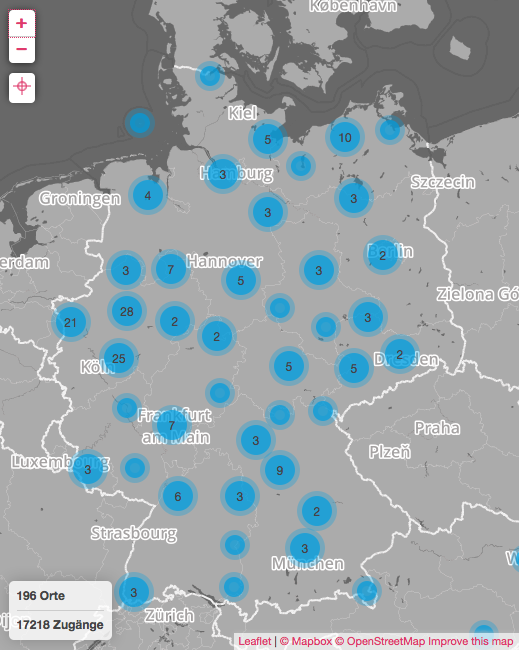
\includegraphics[width=\textwidth]{Bilder/community-map-2015-08-13}
			\end{center}
		\end{column}
	\end{columns}
\end{frame}


%5
\begin{frame}{Knotenkarte}
	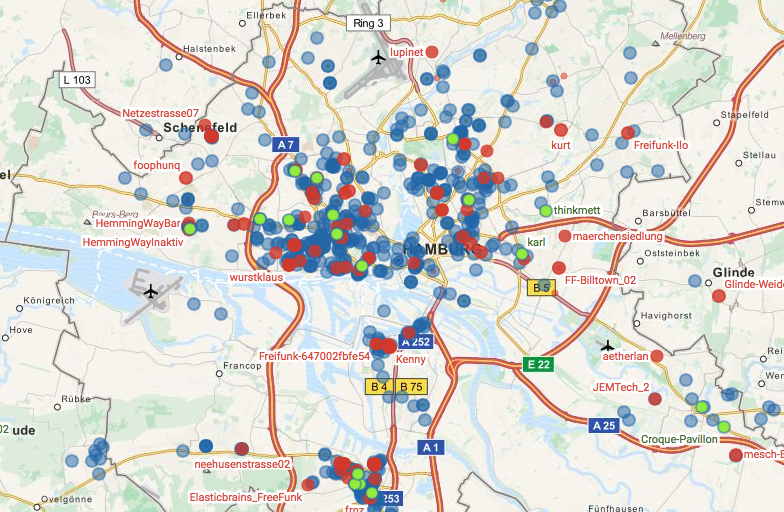
\includegraphics[width=.8\textwidth]{Bilder/knotenkarte-2015-08-13}
	\newline Über 850 Knoten in Hamburg
\end{frame}


%6-9
\begin{frame}{Freifunkknoten}
	\includegraphics[width=.6\textwidth]{Bilder/841}
\end{frame}

\foreach \index in {1, ..., 4} 
{
    \begin{frame}{Das Netzwerk}
        \centering \includesvg[width=9cm]{netz-\index}
    \end{frame}
}


%10
\begin{frame}{Sicherheit}
	\begin{itemize}
		\item Wie bei allen offenen WLANs, ist die Funkstrecke zum Zugangspunkt unverschlüsselt
		\item Wie sonst im Netz auch, sollte nach Möglichkeit Ende-zu-Ende-Verschlüsselung genutzt werden
		\item Freifunk und Heim- / Firmennetz sind getrennt
	\end{itemize}
\end{frame}


%11
\begin{frame}{Haftung}
	\begin{itemize}
		\item Keine Haftung für Knotenbetreiber
		\item Aller Internetverkehr geht durch die Gateways. Diese sind nach TMG\S8 von Haftung befreit.
		\item Wir nehmen die gesetzlichen Vorschriften wörtlich: Wir sammeln keine Daten.
	\end{itemize}
\end{frame}


%12
\begin{frame}{\href{http://wiki.freifunk.net/Freifunk_Hamburg/Richtfunknetz}{Richtfunknetz}}
	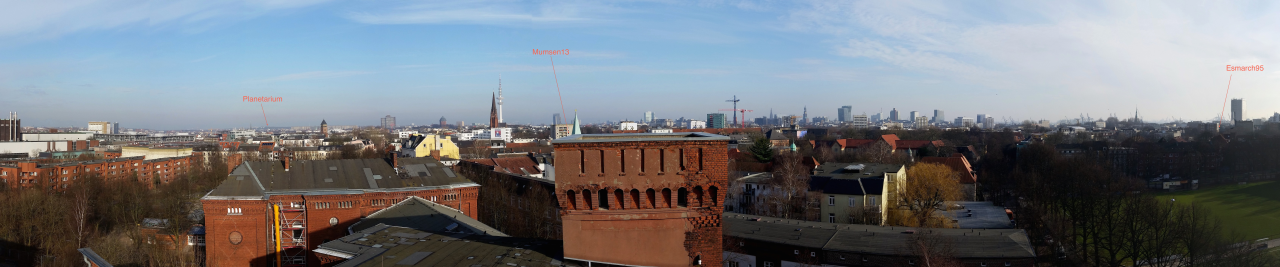
\includegraphics[width=\textwidth]{Bilder/fux}
	\begin{columns}
		\begin{column}{0.7\textwidth}
			\begin{itemize}
				\item Redundanz und Lastverteilung
				\item Unabhängigkeit vom Internet
				\item Demokratieversicherung
			\end{itemize}
		\end{column}
		\begin{column}{0.3\textwidth}
			\begin{center}
				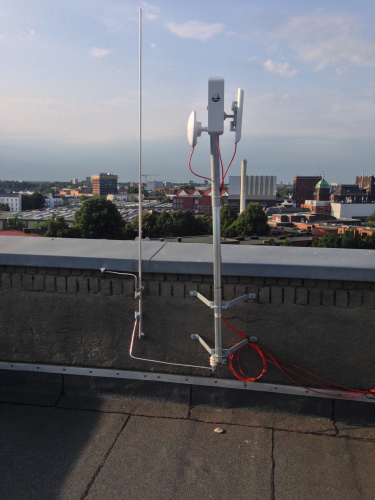
\includegraphics[width=.9\textwidth]{Bilder/richtfunkmast}
			\end{center}
		\end{column}
	\end{columns}
\end{frame}


%13
\begin{frame}{Dienste}
	\begin{itemize}
		\item Internet (IPv4 \& IPv6)
		\item Stadtweites Intranet (IPv4 \& IPv6)
		\item Verbindungen zu anderen Städten und Netzwerken sowie deren Diensten (IP-Telefonie, Videochat...)
		\item Jeden Dienst, den man selbst gerne anbieten möchte
	\end{itemize}
\end{frame}

%14
\begin{frame}{Öffentliche Wahrnehmung}
	\begin{itemize}
		\item Von Neelie Kroes bis Alexander Dobrindt, alle fordern freies Internet - wir machen es.
		\item MABB hat gerade eine 46-seitige \href{http://mabb.de/presse/pressemitteilungen/details/wlan-fuer-alle-freie-funknetze-in-der-praxis.html}{Broschüre über freifunk} herausgegeben 
		\item Überweltigende Medienrezeption unter \href{http://wiki.freifunk.net/Medienspiegel}{http://wiki.freifunk.net/Medienspiegel}
	\end{itemize}
\end{frame}


%15
\begin{frame}{Freifunk lebt vom Mitmachen}
	\begin{itemize}
		\item Stellt Knoten auf
		\item Biete eigene Dienste an
		\item Firmware, Administration, Dokumentation, Grafik, Öffentlichkeitsarbeit
		\item Unterstütze ein Projekt: Flüchtlingshilfe, Richtfunk...
		\item Treffen Montags \& Freitags
	\end{itemize}
\end{frame}

%16
\begin{frame}{\href{http://start.ffhh/}{http://start.ffhh/}}
	\begin{itemize}
		\item Künstlerische Projekte
		\item Radio / Podcast
		\item Verschlüsselter Videochat
		\item Blogs
		\item Dateitausch
		\item SIP Telefonie...
	\end{itemize}
\end{frame}


%16
\begin{frame}{Vielen Dank!}
	\begin{columns}
		\begin{column}{1\textwidth}
			\begin{itemize}
				\item Netz: \href{https:///hamburg.freifunk.net}{https:///hamburg.freifunk.net}
				\item Ansprechpartner im Werkhof: Ulf
				\item Mail: \href{mailto:ulf.treger@dekoder.de}{ulf.treger@dekoder.de}
				\item Treffen 2x/Woche: \href{https://hamburg.freifunk.net/kalender}{https://hamburg.freifunk.net/kalender}
		\end{itemize}
			\begin{center}
				\includegraphics[width=0.2\textwidth]{Bilder/cc-by}
			\end{center}
		\end{column}
	\end{columns}
\end{frame}

\end{document}